\documentclass[11pt,a4paper]{article}

% ---------- EsadeEcPol-inspired policy-brief look ----------
\usepackage[T1]{fontenc}
\usepackage[utf8]{inputenc}
\usepackage{helvet}\renewcommand{\familydefault}{\sfdefault}
\usepackage[margin=2.3cm,top=2.0cm,bottom=2.4cm]{geometry}
\usepackage{graphicx,booktabs,xcolor,tcolorbox,caption,enumitem,setspace}
\usepackage[hidelinks]{hyperref}

\definecolor{ecnavy}{HTML}{12355B}
\definecolor{ecyellow}{HTML}{FFCD00}
\definecolor{eccoral}{HTML}{E34948}
\definecolor{ecblue}{HTML}{2A78D6}
\definecolor{ecink}{HTML}{1A2430}
\definecolor{ecgray}{HTML}{5A6572}
\definecolor{ecpale}{HTML}{FFF8DC}

\captionsetup{font={small},labelfont={bf,color=ecnavy},
              justification=raggedright,singlelinecheck=false}
\makeatletter\setlength{\@fptop}{0pt}\makeatother  % floats start at page top
\setlength{\parskip}{5pt}\setlength{\parindent}{0pt}
\linespread{1.12}
\color{ecink}

\newcommand{\heronum}[2]{%
  \begin{minipage}[t]{0.30\textwidth}\raggedright
  {\fontsize{30}{32}\selectfont\bfseries\color{ecnavy}#1}\\[2pt]
  {\small\color{ecgray}#2}
  \end{minipage}}

\begin{document}

% ---------- cover band ----------
\begin{tcolorbox}[colback=ecyellow,colframe=ecyellow,sharp corners,
                  left=14pt,right=14pt,top=16pt,bottom=16pt]
  \raggedright
  {\small\bfseries\color{ecnavy}POLICY BRIEF \;·\; TEACHER LABOR MARKETS \;·\; JULY 2026}\\[10pt]
  {\fontsize{22}{26}\selectfont\bfseries\color{ecnavy}%
  Who leaves teaching? Two decades of teacher attrition in the United States, 2005--2025\par}\vspace{10pt}
  {\normalsize\color{ecink}Evidence from 174{,}872 school teachers followed for
  twelve months each in linked Current Population Survey microdata}
\end{tcolorbox}

\vspace{10pt}

% ---------- executive summary ----------
\begin{tcolorbox}[colback=ecpale,colframe=ecpale,sharp corners,
                  left=12pt,right=12pt,top=10pt,bottom=10pt]
{\bfseries\color{ecnavy}EXECUTIVE SUMMARY}

\begin{itemize}[leftmargin=14pt,itemsep=2pt]
  \item Because \textbf{one in six 12-month leavers (15.7\%) is back teaching
  within three months}, we define attrition strictly: a \emph{persistent
  leaver} is out of teaching twelve months later \emph{and} in every
  re-interview thereafter. By this measure, \textbf{15.1\% of degree-holding
  school teachers persistently leave the profession each year}: 9.9 percentage
  points (pp) to another occupation, 4.5\,pp out of the labor force, 0.6\,pp
  to unemployment. The conventional 12-month definition gives 17.6\%.
  \item Persistent attrition has \textbf{risen by about four points in two
  decades} --- from ~13\% in 2005--2010 to ~17\% in 2022--2024, with a COVID
  spike (18.4\% in 2019$\to$2020) and a new high of 18.0\% in 2024.
  \item \textbf{Working part-time is by far the strongest predictor} of
  leaving ($+12.2$\,pp). Exit risk is U-shaped in age (lowest at 40) and higher
  for Black ($+5.9$\,pp), non-citizen ($+7.6$\,pp) and preschool/kindergarten
  ($+4.2$\,pp) teachers. Among degree holders, a graduate degree adds only
  modest extra protection ($-1.1$\,pp). All effects are nearly identical under
  the conventional definition --- the predictors are robust.
  \item The \textbf{typical persistent leaver} is a woman in her late career,
  working part-time, without a graduate credential --- the top predicted-risk
  decile faces a 35\% exit probability, 2.4 times the average teacher.
\end{itemize}
\end{tcolorbox}

\vspace{6pt}
\noindent
\heronum{15.1\,\%}{of teachers leave the profession for good each year}\hfill
\heronum{$+$12.2\,pp}{extra exit risk from part-time work}\hfill
\heronum{1 in 6}{12-month leavers is back teaching within 3 months}

\vspace{4pt}
\section*{\color{ecnavy}1. The population we observe --- who can be followed,
and for how long}

We use official \textbf{Current Population Survey (CPS) basic monthly
microdata}: 251 monthly files covering January 2005 to December 2025, from the
U.S. Census Bureau (2024--2025) and the NBER mirror (2005--2023); October 2025
was never released. The CPS interviews each household on a \textbf{4--8--4
rotation} (Figure~\ref{fig:design}): four consecutive months in sample, eight
months out, four months back in --- so any person is observable for at most
\textbf{16 months}, once. Within that window, each adult interviewed in year
$t$ is re-interviewed in the same calendar month of $t{+}1$ and can be linked
by household and person identifiers, with matches validated on sex, race and
age progression (Madrian--Lefgren criterion). No one can be followed across
multiple years: each base year is a \emph{fresh cohort}, which is why every
rate in this brief is computed wave by wave.

\begin{figure}[h!]
  \caption{\textbf{The CPS follows each person for at most 16 months.}
  Interview calendar of one rotation group; numbers are months since first
  interview.}
  \label{fig:design}
  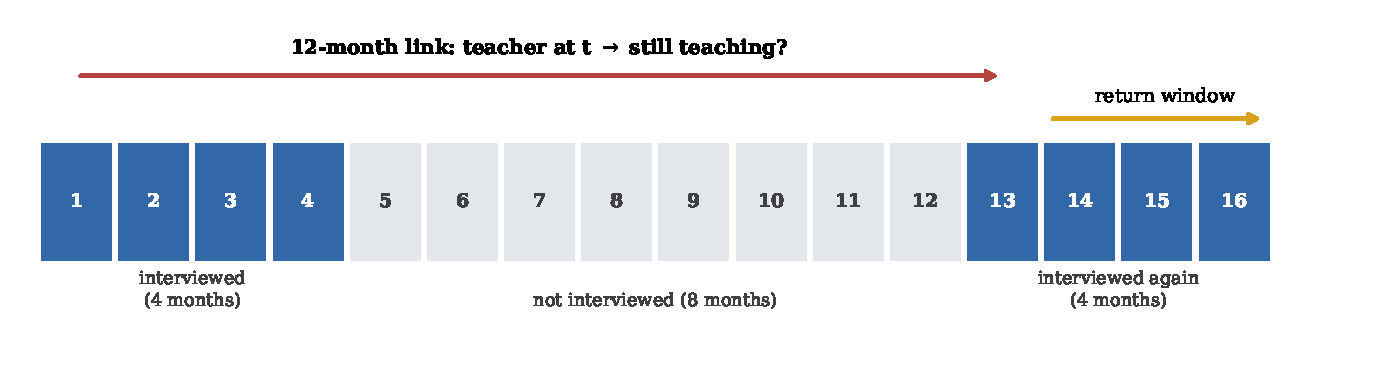
\includegraphics[width=0.95\textwidth]{figures/fig0_design.pdf}
  \par{\footnotesize\color{ecgray}The 12-month link compares months $m$ and
  $m{+}12$ ($m \le 4$); the return window re-observes leavers in months
  $m{+}13$ to 16.}
\end{figure}

Table~\ref{tab:pop} shows the full population funnel, pooling all 251 months.

\begin{table}[h!]
  \caption{\textbf{From the CPS universe to the analytic sample.}}
  \label{tab:pop}
  \centering\small
  \begin{tabular}{lrr}
\toprule
 & Person-months & \% of previous \\
\midrule
Adult interviews (person-months), 2005--2025 & 23,752,044 & -- \\
\quad employed & 14,450,470 & 61\% \\
\quad\quad school teachers (occ. 2300--2330) & 525,651 & 4\% \\
\quad\quad\quad with bachelor's degree or higher & 464,144 & 88\% \\
\quad\quad\quad\quad in a linkable rotation (MIS 1--4) & 229,930 & 50\% \\
\textbf{Linked to their interview 12 months later} & 174,872 & -- \\
\quad with re-interviews after $t{+}12$ (MIS 1--3) $\to$ \textbf{main sample} & 129,897 & 74\% \\
\bottomrule
\end{tabular}

  \par\vspace{4pt}{\footnotesize\color{ecgray}Teachers are identified as
  employed persons whose primary-job occupation is preschool/kindergarten,
  elementary/middle, secondary, or special-education teacher (Census codes
  2300--2330, identical across the 2002, 2010 and 2020 classifications),
  holding a bachelor's degree or higher. Only rotations in months-in-sample
  1--4 can be linked forward; 67\% of linkable teachers are found and
  validated 12 months later.}
\end{table}

\textbf{Defining a leaver.} The conventional measure (\emph{12-month leaver},
as in the NCES Teacher Follow-up Survey) counts anyone not employed as a
school teacher twelve months after baseline. But temporary exits --- parental
leave, short unemployment spells, sabbaticals --- inflate it: re-observing
leavers in their up-to-three remaining monthly interviews, 15.7\% are already
teaching again. Our main measure is therefore the \emph{persistent leaver}:
out of teaching at $t{+}12$ \emph{and} in every subsequent re-interview,
computed on the 129{,}897 teachers whose rotation allows at least one
re-interview. Exits longer than a year that end in a return cannot be
detected --- persistent attrition remains a (much tighter) upper bound on
permanent exit. Rates use CPS final person weights.

\textit{Caveat:} occupation in the returning rotation is re-coded
independently, which inflates measured occupation switching; levels should be
read as upper bounds, while \emph{comparisons across groups and over time} ---
the object of this brief --- are far less affected.

\section*{\color{ecnavy}2. The teacher workforce: stock, composition, flows}

Weighted to population, the CPS counts a stable stock of degree-holding
school teachers (Figure~\ref{fig:stock}), dominated by elementary/middle
school teaching (Figure~\ref{fig:levels}).

\begin{figure}[h!]
  \caption{\textbf{The stock of school teachers.} Estimated number of
  employed school teachers with a bachelor's degree or higher, annual average
  of monthly estimates.}
  \label{fig:stock}
  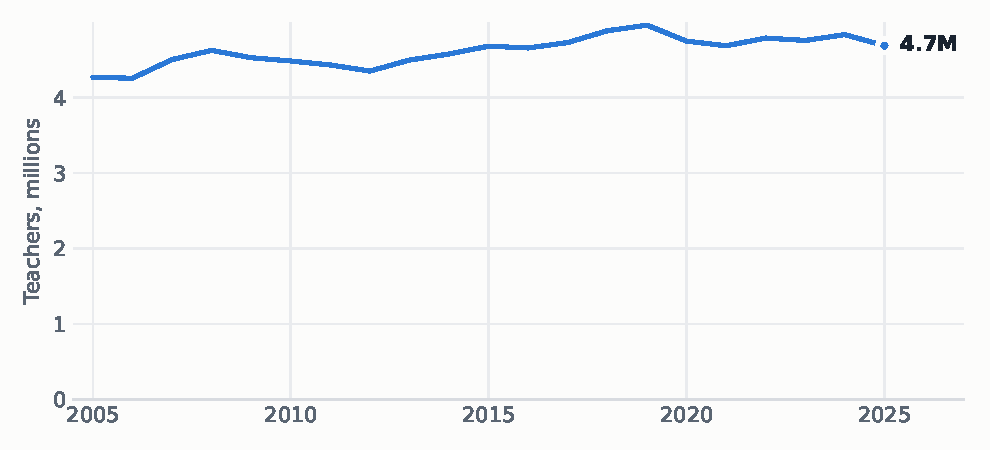
\includegraphics[width=0.80\textwidth]{figures/fig7_stock.pdf}
  \par{\footnotesize\color{ecgray}Source: CPS basic monthly files, person
  weights. Teachers = employed, primary-job occupation codes 2300--2330
  (preschool/kindergarten, elementary/middle, secondary, special education),
  bachelor's degree or higher.}
\end{figure}

\begin{figure}[h!]
  \caption{\textbf{Teachers by teaching level.} Same identification, by
  occupation code.}
  \label{fig:levels}
  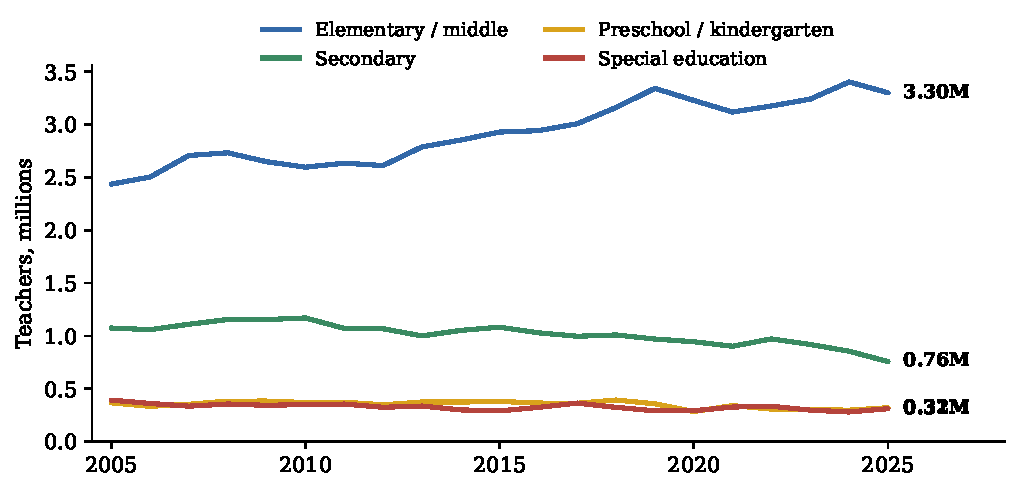
\includegraphics[width=0.84\textwidth]{figures/fig8_by_level.pdf}
  \par{\footnotesize\color{ecgray}Source: CPS basic monthly files, person
  weights.}
\end{figure}

The linked pairs also reveal both sides of the turnover ledger
(Figure~\ref{fig:flows}): the profession simultaneously loses and recruits
15--20\% of its stock every year --- a high-churn occupation in which exits
have been trending above entries in recent years.

\begin{figure}[h!]
  \caption{\textbf{Teaching loses and recruits 15--20\% of its stock every
  year.} Gross annual flows into and out of school teaching, linked pairs
  (12-month definitions).}
  \label{fig:flows}
  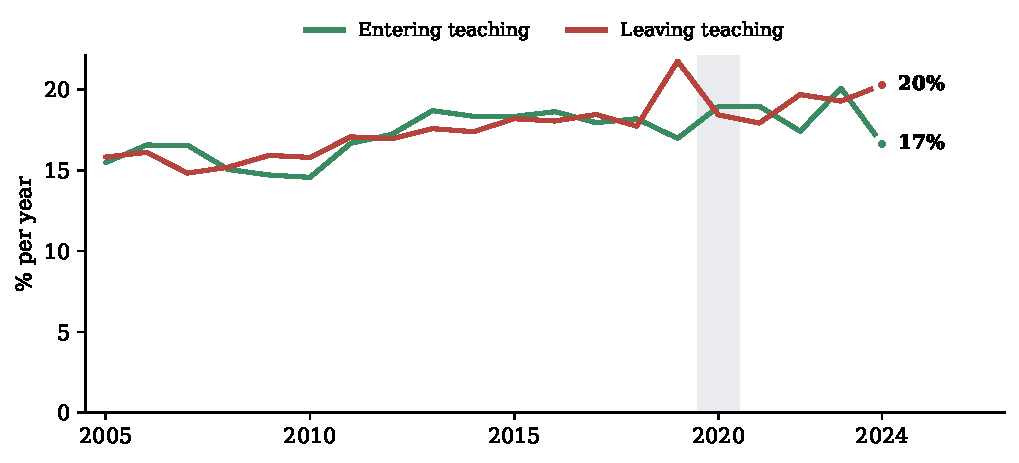
\includegraphics[width=0.84\textwidth]{figures/fig9_flows.pdf}
  \par{\footnotesize\color{ecgray}Source: linked CPS pairs. Entering = school
  teacher (BA+) at $t{+}12$ who was not a school teacher at $t$; leaving =
  the reverse. Linked samples under-count movers, so both flows are
  conservative.}
\end{figure}

\begin{figure}[h!]
  \caption{\textbf{Most persistent leavers move to other jobs rather than out
  of work.} Destination of persistent leavers, share of baseline teachers
  (weighted), 2005--2025.}
  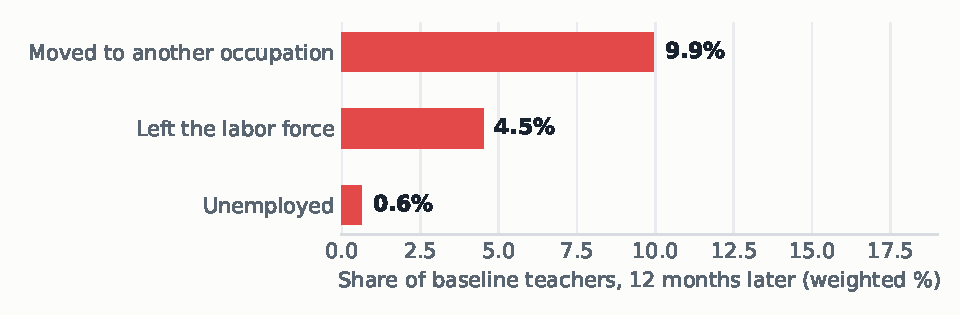
\includegraphics[width=0.82\textwidth]{figures/fig1_destinations.pdf}
  \par{\footnotesize\color{ecgray}Source: authors' calculations, linked CPS
  basic monthly files 2005--2025.}
\end{figure}

\section*{\color{ecnavy}3. Attrition is rising --- and part of it is churn}

One in six 12-month leavers is teaching again within three months (women
16.1\%, men 14.0\%; Figure~\ref{fig:evol}, right) --- temporary exits that the
persistent definition strips out. Net of this churn, \textbf{persistent
attrition still climbed from ~13\% in 2005--2010 to ~17\% in 2022--2024}
(Figure~\ref{fig:evol}, left), peaking in the pandemic year (18.4\% in
2019$\to$2020) and reaching a new high of 18.0\% in 2024. Gender gaps are
small and unstable; in the most recent year men (19.8\%) exceeded women
(17.4\%).

\begin{figure}[h!]
  \caption{\textbf{Persistent attrition has risen four points in two decades;
  one in six 12-month leavers returns within three months.} Weighted rates by
  base year and gender.}
  \label{fig:evol}
  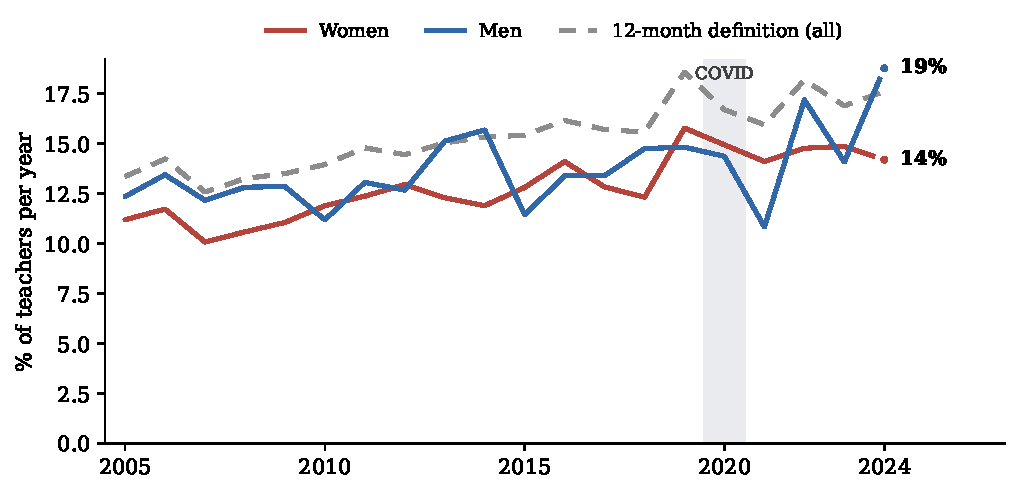
\includegraphics[width=\textwidth]{figures/fig6_evolution.pdf}
  \par{\footnotesize\color{ecgray}Source: authors' calculations, linked CPS
  2005--2025. Return window truncated by the CPS design at three monthly
  interviews after $t{+}12$ (leavers re-interviewed at least once:
  21{,}873 of 30{,}244).}
\end{figure}

\section*{\color{ecnavy}4. Who leaves: raw differences}

Attrition concentrates in three margins: \textbf{hours}, \textbf{teaching
level} and, more weakly once degree holders only are considered,
\textbf{credentials}. Part-time teachers leave at more than twice the rate of
full-time teachers; preschool/kindergarten is the most exposed level.

\begin{figure}[h!]
  \caption{\textbf{Attrition more than doubles without full-time hours.}
  Weighted persistent attrition rate by baseline characteristics, 2005--2025.}
  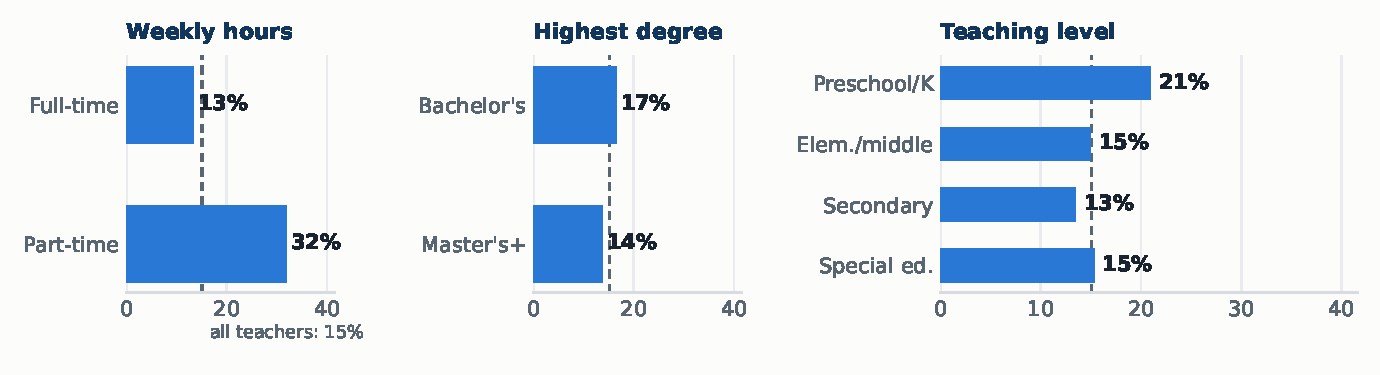
\includegraphics[width=\textwidth]{figures/fig2_rates_by_group.pdf}
  \par{\footnotesize\color{ecgray}Source: authors' calculations, linked CPS
  2005--2025. Dashed line: all-teacher average (15.1\%).}
\end{figure}

\section*{\color{ecnavy}5. A probit model of leaving teaching}

We estimate a probit for the probability of \emph{persistently} leaving, with
covariates measured at baseline, base-year fixed effects, and standard errors
clustered by household (Table~\ref{tab:probit}); Figure~\ref{fig:ame} plots
the average marginal effects. Three results stand out. First, \textbf{part-time
status raises exit probability by 12.2\,pp}, the largest effect in the model by
an order of magnitude --- attachment to full-time hours, not demographics, is
the dominant margin. Second, \textbf{minority and non-citizen teachers are
significantly more likely to leave} (Black $+5.9$\,pp, non-citizen
$+7.6$\,pp, Hispanic $+1.5$\,pp), a retention gap with direct implications for
workforce diversity. Third, among degree holders \textbf{a graduate degree
adds only $-1.1$\,pp of protection}, while higher family income ($-2.5$\,pp),
teaching secondary school ($-0.8$\,pp) and being a woman ($-0.9$\,pp) also
retain modestly. Every effect is nearly identical under the conventional
12-month definition (largest difference: part-time, $+14.5$ vs $+12.2$\,pp)
--- the predictors are not an artifact of how leaving is measured.

\begin{figure}[h!]
  \caption{\textbf{Hours dominate demographics.} Average marginal effects on
  the probability of leaving teaching within 12 months, with 95\% confidence
  intervals.}
  \label{fig:ame}
  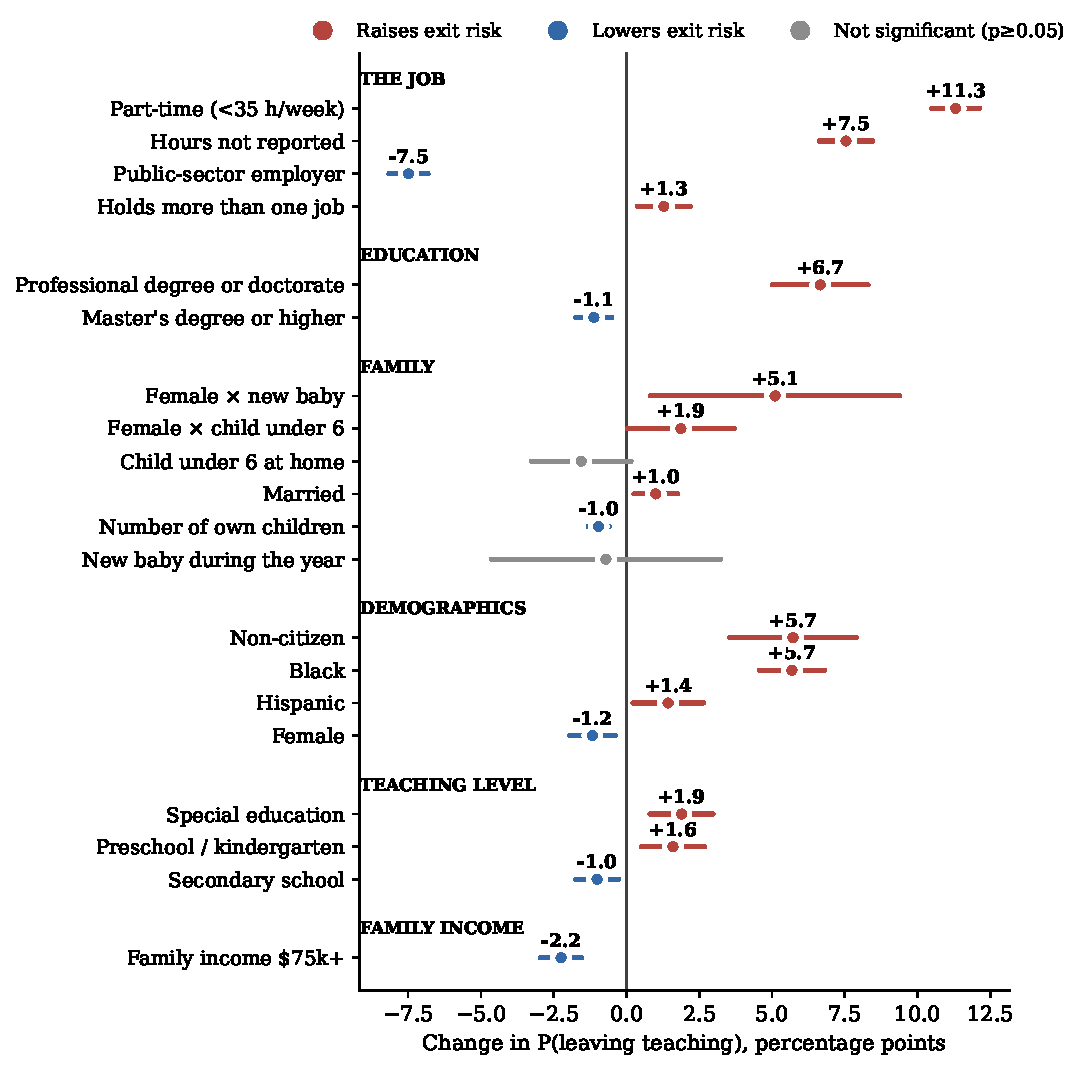
\includegraphics[width=0.94\textwidth]{figures/fig3_ame.pdf}
  \par{\footnotesize\color{ecgray}Source: probit of Table~\ref{tab:probit}.
  Age terms shown in Figure~\ref{fig:age}.}
\end{figure}

Age enters with a robust U-shape (Figure~\ref{fig:age}): predicted risk falls
to a minimum of 9\% around age 39 and accelerates after 55 as retirement
margins open, reaching 28\% at 70 --- the familiar U-shaped attrition profile
of the teacher-turnover literature.

\begin{figure}[h!]
  \caption{\textbf{Exit risk is U-shaped in age, lowest near 40.} Predicted
  probability of leaving by age, other covariates at sample means; shaded band:
  95\% CI.}
  \label{fig:age}
  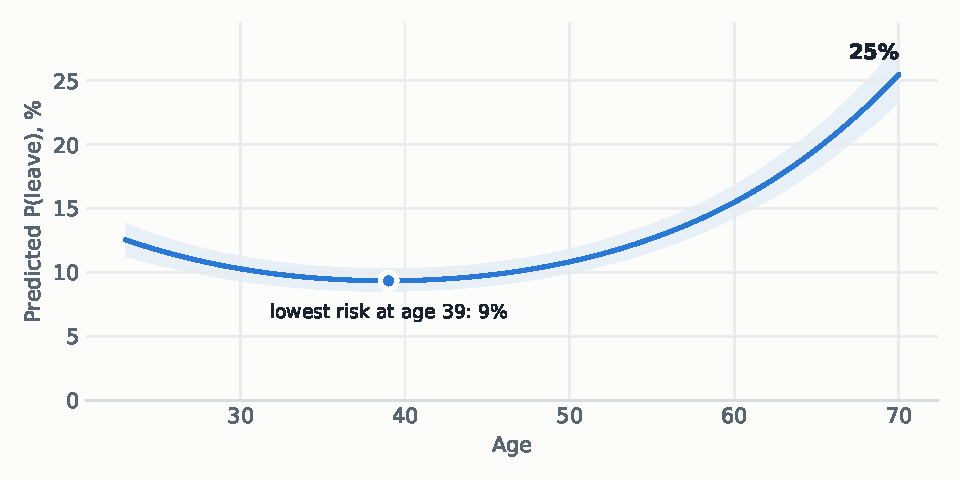
\includegraphics[width=0.80\textwidth]{figures/fig4_age_profile.pdf}
  \par{\footnotesize\color{ecgray}Source: probit of Table~\ref{tab:probit},
  simulation-based confidence band.}
\end{figure}

\begin{table}[h!]
  \caption{\textbf{Probit estimates: probability of persistently leaving
  teaching, 2005--2025.}}
  \label{tab:probit}
  \centering\small
  \begin{tabular}{lccc}
\toprule
 & Probit coef. & (SE) & AME (pp) \\
\midrule
Age (years) & -0.055$^{***}$ & (0.004) & -1.18$^{***}$ \\
Age$^2$/100 & 0.070$^{***}$ & (0.004) & +1.50$^{***}$ \\
Female & -0.049$^{***}$ & (0.018) & -1.05$^{***}$ \\
Married & 0.055$^{***}$ & (0.018) & +1.18$^{***}$ \\
Number of own children & -0.047$^{***}$ & (0.009) & -1.00$^{***}$ \\
Child under 6 at home & -0.076$^{*}$ & (0.041) & -1.63$^{*}$ \\
Female $\times$ child under 6 & 0.087$^{**}$ & (0.044) & +1.88$^{**}$ \\
Black & 0.265$^{***}$ & (0.027) & +5.68$^{***}$ \\
Hispanic & 0.067$^{**}$ & (0.029) & +1.44$^{**}$ \\
Non-citizen & 0.267$^{***}$ & (0.052) & +5.72$^{***}$ \\
Master's degree or higher & -0.051$^{***}$ & (0.015) & -1.09$^{***}$ \\
Professional degree or doctorate & 0.311$^{***}$ & (0.039) & +6.66$^{***}$ \\
Part-time ($<$35 h/week) & 0.527$^{***}$ & (0.020) & +11.30$^{***}$ \\
Hours not reported & 0.352$^{***}$ & (0.022) & +7.54$^{***}$ \\
Holds more than one job & 0.060$^{***}$ & (0.021) & +1.28$^{***}$ \\
Public-sector employer & -0.349$^{***}$ & (0.016) & -7.49$^{***}$ \\
Family income \$75k+ & -0.105$^{***}$ & (0.017) & -2.24$^{***}$ \\
Midwest & -0.082$^{***}$ & (0.021) & -1.75$^{***}$ \\
South & 0.008 & (0.020) & +0.16 \\
West & -0.016 & (0.021) & -0.35 \\
Preschool / kindergarten & 0.075$^{***}$ & (0.026) & +1.61$^{***}$ \\
Secondary school & -0.047$^{***}$ & (0.018) & -1.01$^{***}$ \\
Special education & 0.088$^{***}$ & (0.026) & +1.89$^{***}$ \\
\midrule
Constant & 0.140 & (0.095) & \\
Base-year fixed effects & \multicolumn{3}{c}{Yes} \\
Observations & \multicolumn{3}{c}{129,897} \\
Pseudo $R^2$ & \multicolumn{3}{c}{0.068} \\
\bottomrule
\end{tabular}

  \par\vspace{4pt}{\footnotesize\color{ecgray}Outcome: persistent leaver.
  Cluster-robust standard errors (by household) in parentheses. AME: average
  marginal effect in percentage points. Sample: school teachers with a
  bachelor's degree or higher and a potential post-$t{+}12$ re-interview
  (baseline MIS 1--3). Reference categories: full-time, bachelor's degree,
  elementary/middle school. $^{***}p<0.01$, $^{**}p<0.05$, $^{*}p<0.1$.}
\end{table}

\section*{\color{ecnavy}6. The profile of the typical leaver}

Ranking teachers by predicted risk, the top decile --- with a mean persistent
exit probability of 35\%, against 15\% for the average teacher --- is
overwhelmingly female (80\%), in the late-career age range (mean 56), seven
times more likely to work part-time (64\% vs.\ 9\%), less likely to hold a
graduate degree (40\% vs.\ 52\%), and over twice as concentrated in
preschool/kindergarten (20\% vs.\ 8\%), with Black teachers over-represented
(14\% vs.\ 6\%).

\begin{figure}[t!]
  \caption{\textbf{The highest-risk teacher: part-time, less credentialed,
  early-years.} Characteristics of the top predicted-risk decile vs.\ all
  teachers.}
  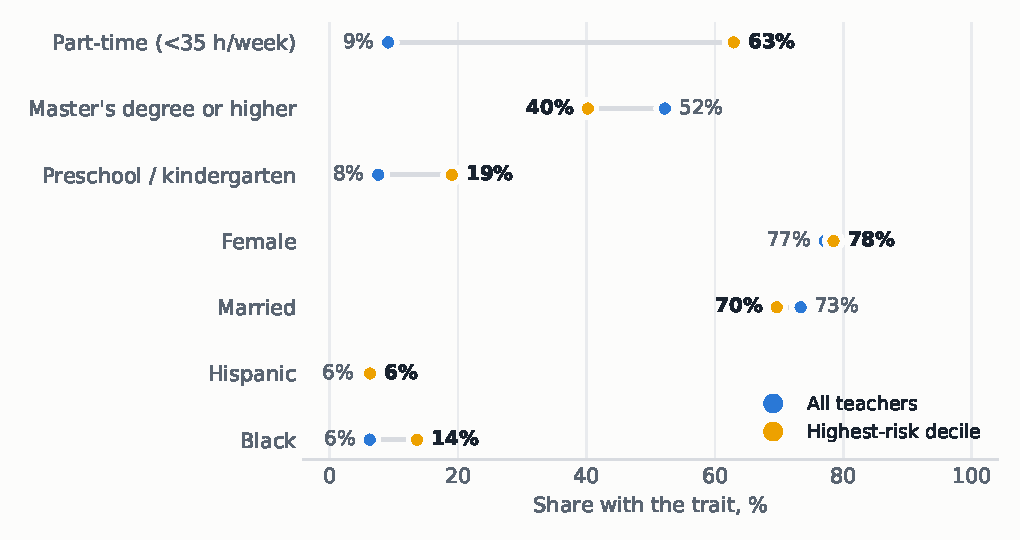
\includegraphics[width=0.92\textwidth]{figures/fig5_profile.pdf}
  \par{\footnotesize\color{ecgray}Source: predicted probabilities from the
  probit of Table~\ref{tab:probit}.}
\end{figure}

\section*{\color{ecnavy}7. Policy implications}

The results locate teacher attrition in \textbf{weak attachment} --- part-time
hours, the early-childhood segment, both career extremes --- rather than in
broad demographics, and show a \textbf{structurally rising trend} since the
early 2010s. Four levers follow. (i) \textbf{Full-time conversion} of
involuntary part-time positions attacks the single largest risk factor.
(ii) \textbf{Retention packages for preschool and kindergarten teachers}, the
most exposed level. (iii) The significant \textbf{Black, Hispanic and
non-citizen retention gaps} warrant targeted monitoring, since they compound
into the diversity of the future workforce. (iv) With \textbf{one in six
leavers back within three months}, cheap re-entry pathways --- fast-track
rehiring, credential portability across districts, return bonuses --- can
recover part of the outflow at low cost.

\vspace{8pt}
\begin{tcolorbox}[colback=ecnavy,colframe=ecnavy,sharp corners,
                  left=12pt,right=12pt,top=8pt,bottom=8pt]
{\small\color{white}\textbf{Methods in one line.} Twenty linked CPS 4--8--4
rotation panels, 2005$\to$2025 · 174{,}872 teachers (129{,}897 with follow-up)
· persistent-leaver outcome · probit, year FE, household-clustered SE · fully
reproducible: \texttt{src/02\_build\_cps\_panel.py} $\to$
\texttt{src/05\_evolution.py} $\to$ \texttt{src/03\_model\_attrition.py}.}
\end{tcolorbox}

\end{document}
